
\documentclass[paper=a4,DIV15,oneside,lefteqn,american]{scrartcl}
\pdfoutput=1

\usepackage[american,german]{babel} 
\usepackage[margin=1.2in]{geometry}

\usepackage[T1]{fontenc}
\usepackage[utf8]{inputenc}

\usepackage{hyperref}
\usepackage[pdftex]{graphicx}
\usepackage{xspace}
\usepackage{textcomp}
\usepackage{framed}

\usepackage[draft,inline,nomargin]{fixme}

\usepackage{verbatim}

\usepackage{amsmath}
\usepackage{amssymb}
\usepackage{amsthm}
\usepackage{txfonts}
\usepackage{mathtools}

\addtolength{\parskip}{0.5\baselineskip}
\parindent=0cm



\newcommand{\VV}{Verification \& Validation\xspace}
\newcommand{\vv}{verification \& validation\xspace}

\def\CC{{C\nolinebreak[4]\hspace{-.05em}\raisebox{.4ex}{\tiny\bf ++}}}

\newcommand{\adhesion}{\mbox{\inl{AdhesionFactor}}\xspace}

\newcommand{\bitwalker}{\mbox{\texttt{Bitwalker}}\xspace}

\newcommand{\poke}{\mbox{\texttt{Bitwalker\_Poke}}\xspace}
\newcommand{\peek}{\mbox{\texttt{Bitwalker\_Peek}}\xspace}
\newcommand{\acsl}{\mbox{\textsf{ACSL}}\xspace}
\newcommand{\isoc}{\mbox{\textsf{C}}\xspace}
\newcommand{\framac}{\mbox{\textsf{Frama-C}}\xspace}
\newcommand{\framacwp}{\mbox{\textsf{Frama-C\slash WP}}\xspace}
\newcommand{\why}{\mbox{\textsf{Why}}\xspace}
\newcommand{\wpframac}{\mbox{\textsf{WP}}\xspace}
\newcommand{\altergo}{\mbox{\textsf{Alt-Ergo}}\xspace}
\newcommand{\qed}{\mbox{\textsf{Qed}}\xspace}
\newcommand{\cvc}{\mbox{\textsf{CVC4}}\xspace}
\newcommand{\z}{\mbox{\textsf{Z3}}\xspace}
\newcommand{\coq}{\mbox{\textsf{Coq}}\xspace}
\newcommand{\cealist}{\mbox{\textsf{CEA LIST}}\xspace}
\newcommand{\fokus}{\mbox{\textsf{Fraunhofer FOKUS}}\xspace}

\newcommand{\inl}[1]{\lstinline[style=inline]{#1}}


%Defining C-Code Environment

\usepackage{courier} 
\usepackage{listings}
\usepackage{color} 

% fix bug with listing under texlive-2014
% see https://lists.debian.org/debian-tex-maint/2014/06/msg00209.html

\makeatletter
\renewcommand\lstinline[1][]{%
  \leavevmode\bgroup % \hbox\bgroup --> \bgroup
  \def\lst@boxpos{b}%
  \lsthk@PreSet\lstset{flexiblecolumns,#1}%
  \lsthk@TextStyle
  \ifnum\iffalse{\fi`}=\z@\fi
  \@ifnextchar\bgroup{%
  \ifnum`{=\z@}\fi%
  \afterassignment\lst@InlineG \let\@let@token}{%
  \ifnum`{=\z@}\fi\lstinline@}}
\makeatother


%\definecolor{darkred}		{rgb}{0.60,0.00,0.00}
\definecolor{coACSLBehavior}	{rgb}{0.30,0.00,0.00}
\definecolor{coASCL}		{rgb}{0.00,0.10,0.00}
\definecolor{coASCLKeyword}	{rgb}{0.00,0.10,0.10}
\definecolor{darkgreen}		{rgb}{0.00,0.40,0.00}
%\definecolor{red}		{rgb}{0.98,0.00,0.00}
\definecolor{darkblue}		{rgb}{0.00,0.00,0.60}
%\definecolor{lightblue}		{rgb}{0.60,0.80,1.00}
%\definecolor{lightred}		{rgb}{1.00,0.60,0.60}
\definecolor{coCKeyword}	{rgb}{0.00,0.00,0.60}

\lstdefinestyle{acsl-block}
{	emph=[1]{assert, assumes, assigns, axiom, axiomatic, decreases, ensures,
                 ghost, invariant, lemma, logic, loop, predicate,
		 reads, requires, variant},
	emphstyle=[1]{\bfseries\color{coASCLKeyword}},
	emph=[2]{behavior, behaviors, complete, disjoint, for:},
	emphstyle=[2]{\bfseries\color{coACSLBehavior}},
	emph=[3]{typedef, int, char, integer, real, bool, size_type, value_type, uint8_t,  uint64_t},
	emphstyle=[3]{\bfseries\color{coCKeyword}},
	escapeinside={//`}{`//},
	morecomment=*[l][\color{coASCL}]{//@},
	morecomment=*[s][\color{coASCL}]{/*@}{*/},
	moredelim=*[is][\bfseries]{|*}{*|},
	%emphstyle=[3]{\ttfamily}
	}

\lstdefinestyle{func-decl}
{	emph=[1]{assert, assumes, assigns, axiom, axiomatic, decreases, ensures,
                 ghost, invariant, lemma, logic, loop, predicate,
		 reads, requires, variant},
	emphstyle=[1]{\bfseries\color{coASCLKeyword}},
	emph=[2]{behavior, behaviors, complete, disjoint, for:},
	emphstyle=[2]{\bfseries\color{coACSLBehavior}},
	emph=[3]{integer, real, size_type, value_type},
	emphstyle=[3]{\bfseries\color{coCKeyword}},
	escapeinside={//`}{`//},
	morecomment=*[l][\color{coASCL}]{//@},
	morecomment=*[s][\color{coASCL}]{/*@}{*/},
	moredelim=*[is][\bfseries]{|*}{*|},
    frame=none,
    numbers=none
	%emphstyle=[3]{\ttfamily}
	}

\lstdefinestyle{acsl-inline}
{	emph=[1]{assert,assigns, assumes, axiom, axiomatic, decreases, ensures, ghost, invariant, lemma, logic, loop,
             predicate, reads, requires, return, variant },
	emphstyle=[1]{\bfseries\color{coASCLKeyword}},
	emph=[2]{behavior, behaviors, complete, disjoint, for:},
	emphstyle=[2]{\bfseries\color{coACSLBehavior}},
	emph=[3]{typedef, int, char, integer, real, bool, size_type, value_type, uint8_t,  uint64_t},
	emphstyle=[3]{\bfseries\color{coCKeyword}},
	morecomment=*[l][\color{coASCL}]{//@},
	morecomment=*[s][\color{coASCL}]{/*@}{*/},
	moredelim=*[is][\bfseries]{|*}{*|}
}

\lstdefinestyle{inline}
{      % basicstyle = \ttfamily\small\color{coASCL},
	keywordstyle = \ttfamily\normal\color{coASCL},
	stringstyle=\color{coASCL},
	style=acsl-inline,
	breaklines= false
}

\lstset{%
  language=C++,
  defaultdialect=ansi,
  basicstyle=\footnotesize\ttfamily,
  commentstyle=\small\color{darkgreen},
  keywordstyle=\small\bfseries\color{darkblue},
  stringstyle=\small\color{darkgreen},
  tabsize = 2,
  showspaces=false,
  showtabs=false,
  columns=fixed,  
  frame=none,  
  breaklines=true,
  showstringspaces=false,
  xleftmargin=0.2cm,
  %rangeprefix=//label, % to specify a certain range from a file
  %rangesuffix=;, % to be shown
  %includerangemarker=false,
	numbers=none
}


\title{Informal Specification of \bitwalker}
\author{Jens Gerlach\\
        {\small Fraunhofer FOKUS, Berlin, Germany}
       }
\date{}

\begin{document}
\selectlanguage{american}
\maketitle
\thispagestyle{empty}
In this technical report a detailed model description of a train control system application is given. The application consists of the ceiling speed monitoring (CSM) function for the European Vital Computer which is the main onboard controller for trains conforming to the European Train Control System specification. The model is provided in SysML, and it is equipped with a formal semantics that is consistent with the (semi formal) SysML standard published by the Object Management Group (OMG). The model and its description are publicly available on http://www.mbt-benchmarks.de, a website dedicated to the publication of models that are of interest for the model-based testing (MBT) community, and may serve as benchmarks for comparing MBT tool capabilities. The model described here is of particular interest for analysing the capabilities of equivalence class testing strategies. The CSM application inputs velocity values from a domain which could not be completely enumerated for test purposes with reasonable effort. 
We describe a novel method for equivalence class testing that -- despite the conceptually infinite cardinality of the input domains -- is capable to produce finite test suites that are exhaustive under certain hypotheses about the internal structure of the system under test.
\tableofcontents
\clearpage
\listoffixmes

\section{Introduction}\label{sec:intro}
% ==========================================================================

\subsection{A Test Model for the ETCS Ceiling Speed Monitor}
In 2011 the {\it model-based testing benchmarks website} www.mbt-benchmarks.org has been 
created with the objective to publish test models that may serve as challenges or benchmarks 
for validating testing theories   and for comparing the capabilities of model-based testing (MBT) tools~\cite{pel2011a}.
In this technical report a novel contribution to this website is presented, a SysML model
of the Ceiling Speed Monitor (CSM) which is part of the European Vital Computer (EVC), the onboard controller of trains conforming to the European Train Control System (ETCS) standard~\cite{ETCS}. In    Section~\ref{sec:ceil} the functional objectives for the CSM are described, and in Section~\ref{sec:modeldesc} the detailed model description is provided. 

The static and behavioural semantics of SysML models have been defined in~\cite{SysML12,uml_2_4} in a semi-formal way, leaving certain ``semantic variation points'' open, so that they can be adjusted according to project-specific requirements. For automated model-based testing, however, a strictly formal semantics is required, so that concrete test data can be calculated from the model's transition relation using constraint solving techniques~\cite{peleska2013ictss}. 
We therefore describe in Section~\ref{sec:transrel} how a formal behavioural semantics is derived for the CSM model and present the associated transition relation in propositional form.

We use state transition systems (STS) for encoding the operational semantics of concrete
modelling formalisms like SysML. STS are widely known from the field of model checking~\cite{clarke_em-etal:1999a}, because their extension into Kripke Structures allows for effective data abstraction techniques. The latter are also applied for equivalence class testing. 
Since state transition systems are a means for semantic representation, testing theories elaborated for STS are applicable for all concrete formalisms whose behavioural semantics can be expressed by STS. In~\cite{d341} it is shown how the semantics of general SysML models and models of a process algebra are encoded as STS. In this technical report we illustrate  how this is achieved for the concrete case of the CSM SysML model.

% ==========================================================================
\subsection{Equivalence Class Partition Testing for the CSM}

The CSM represents a specific test-related challenge: its behaviour depends on actual and allowed speed, and these have conceptually real-valued data domains, so that -- even when   discretising
the input space -- it would be infeasible to exercise all possible combinations of 
inputs on the system under test (SUT). Therefore equivalence class partition (ECP)
 testing strategies have 
to be applied for testing the CSM. While these strategies are well-adopted  in a heuristic manner
in today's industrial test campaigns, practical application of equivalence class testing still lacks 
formal justification of the equivalence classes selected and the sequences of class representatives 
selected as test cases: standard text books used in industry, for example~\cite{spillner2006}, 
only explain the generation of input equivalence class tests for   systems, where the 
SUT reaction to an input class representative is independent on the internal state. Moreover, the systematic calculation of classes from models, as well as their formal justification with respect to
test strength and coverage achieved, is not yet part of today's best practices in industry. 

In contrast to this, formal approaches to equivalence class testing have been studied in the formal methods communities; references to these results  are given in Section~\ref{sec:related}.
In the second main part of this report (Section~\ref{sec:iecpstart}) we therefore describe a recent formal technique for equivalence class testing and its application to testing the CSM. The theoretical 
foundations of this strategy have been published by two of the authors in~\cite{peleska2013ictss}. 
This technical report illustrates its practical application and presents first evaluation details using a 
prototype implementation in an existing MBT tool; the ECP tests are  compared to test results obtained when applying other MBT coverage strategies, such as transition cover or MC/DC coverage (Section~\ref{sec:conventionaltests}). 


% ==========================================================================
\subsection{Fault Models and Completeness Results}


Our ECP strategy
introduces test suites depending on {\it fault models}. This well adopted notion has first been 
introduced in the field of finite state machine (FSM) testing~\cite{petrenko1996}, but is also applicable
to other formal modelling techniques. A fault model consists of a reference model, a conformance relation and a fault domain. The latter is a collection of models whose behaviour may or may not be
consistent to the reference model in the sense of the conformance relation. The test suites generated 
by the ECP strategy described here are {\it complete} with respect to the given fault model: each
system of the fault domain which conforms to the reference model will pass all the generated tests
(this means that the test suite is {\it sound}), and each system in the fault domain that violates the
conformity to the reference model will fail at least  once when tested according to the test suite (the test suite is {\it exhaustive}). 




%%% @todo open proof strategy of the openETCS project







In the following, we present the informal 
specification that Fraunhofer FOKUS derived from analysing the 
implementation of \bitwalker.

\subsection{Basic concepts}

First we introduce various terms that we will use in our informal specifications.
In particular, we distinguish between \emph{bit streams} and \emph{bit sequences}.

\begin{itemize}
\item
A \emph{bit stream} is an array containing elements of type \verb"uint8_t".

\item
If \inl{a} is the starting address of a bit stream and
if all pointers \inl{a+[0..n-1]} are \emph{valid} in the sense
of the \isoc standard (cf.~\cite[\S~6.5.3.2(4)]{ISO:C99}),
then we refer to \inl{a} as a \emph{valid bit stream of length \inl{n}}.

\item 
A bit stream of length $n$ contains $8n$ bits.

\item 
A bit stream can be indexed both by array indices
and \emph{bit indices}.

Figure~\ref{fig:bitstream-indices} shows the difference between 
array indices (bottom row) and bit indices (top row) in a bit stream.
The two bit indices, 0~and~14,
mark bit positions in the first and second array element, respectively.

\begin{figure}[hbt]
\begin{center}
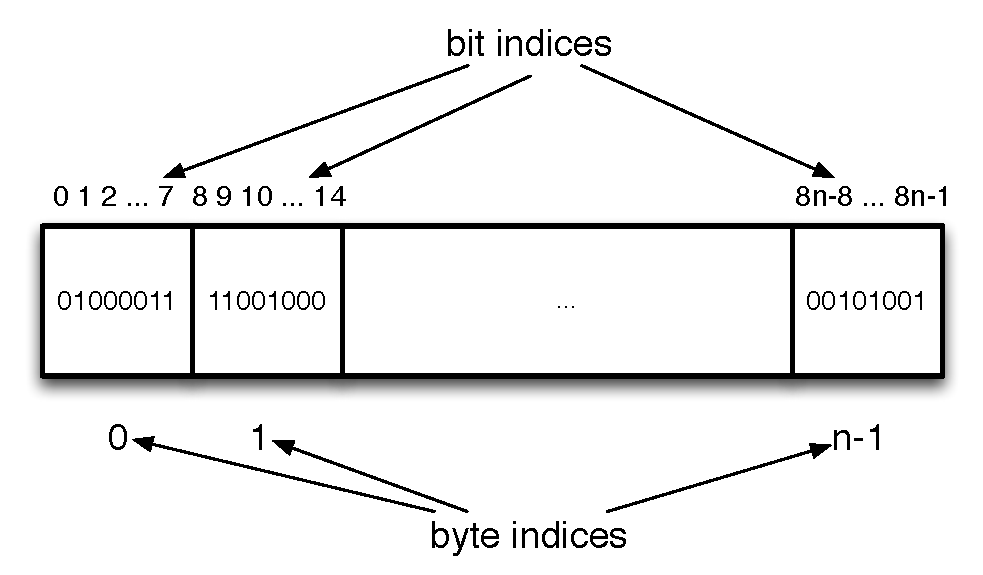
\includegraphics[width=0.65\textwidth]{figures/byte-and-bit-indices.pdf}
\caption{\label{fig:bitstream-indices} Byte indices and bit indices in a bit stream}
\end{center}
\end{figure}


\item 
The C~programming language neither provides a type \emph{bit}
nor does it support random access to the bits of a bit stream.
In order to access the $i$-th bit of a bit sequence one typically
has to first access the byte with index $j = i/8$ and then access the 
bit $k = i \% 8$ within this byte.
Note that in Figure~\ref{fig:bitstream-indices} 
bytes and bits are indexed in increasing order, starting from the \emph{left}.
In big-endian mode, however, bits are indexed from the \emph{right}.
For example, to access the $k$-th bit (from the left) of a byte \inl{a} one can
shift this byte to the right by $7-k$ bits and then extract the now
rightmost bit by performing a bit-wise \emph{and} with the value~1
%
\begin{verbatim}
   (a >> (7-k)) & 1        // get the k-th left-most bit of a
\end{verbatim}

\item
A \emph{bit sequence} is a consecutive sequence of bits within a bit stream
as represented in Figure~\ref{fig:bitsequence}.
\begin{figure}[hbt]
\begin{center}
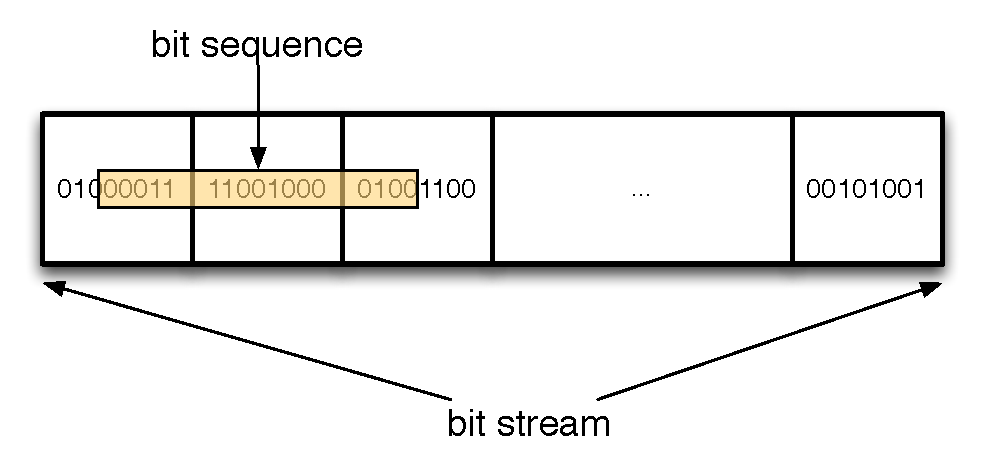
\includegraphics[width=0.65\textwidth]{figures/bit_sequence.pdf}
\caption{\label{fig:bitsequence} A bit sequence within a bit stream}
\end{center}
\end{figure}

A bit sequence is given by the position of its first bit (a bit index in the bit stream)
and its \emph{length}, that is, the number of bits it contains.

\item

A bit sequence that starts at bit index $p$ and has
length $l \geq 0$ is considered \emph{valid} (with respect to a bit stream of length $n$)
if the following conditions are satisfied
\begin{align*}
  0 &\leq p < 8n \\
  0 &\leq p + l \leq 8n
\end{align*}

Note that only the bits with indices $p \leq i < p + l$ are to be accessed
but not the bit with index~$p+l$.

\end{itemize}

We assume that the C-types \inl{unsigned int} and \inl{int}, which
are used in the implementation to represent indices, counting and error codes,
have a width of~32~bits.
We point this out here because we conducted the verification on a platform with
these characteristics.

As an aside, MISRA-C discourages the use of ``generic'' integer types
such as \inl{int} and \inl{unsigned int} and recommends the use of integer types whose names
contain the exact width.


\include{bitwalker-public}
\include{bitwalker-private}

\end{document}
